\subsection*{Problema 13}

\textbf{Enunciado:} 
Calcular la integral indefinida:
\begin{equation*}
\int \frac{1}{x \sqrt{1 + x - x^2}} \, dx
\end{equation*}

\textbf{Solución:} 
Para resolver la integral dada, aplicamos la 
sustitución recíproca sugerida, definiendo 
la nueva variable $u$ como:
\begin{equation*}
u = \frac{1}{x} \implies x = \frac{1}{u}
\end{equation*}

A partir de esta relación, el diferencial 
de $x$ se expresa como:
\begin{equation*}
dx = -\frac{1}{u^2} \, du
\end{equation*}

Sustituimos $x$ y $dx$ en la integral 
original. Notamos que $x$ en el denominador 
se convierte en $1/u$, y el término dentro 
del radical se transforma algebraicamente:
\begin{align*}
1 + x - x^2 &= 1 + \frac{1}{u} - \left(\frac{1}{u}\right)^2 \\
&= 1 + \frac{1}{u} - \frac{1}{u^2} \\
&= \frac{u^2 + u - 1}{u^2}
\end{align*}

Reemplazamos estos componentes 
dentro de la integral:
\begin{align*}
\int &\frac{1}{\left(\frac{1}{u}\right) 
\sqrt{\frac{u^2 + u - 1}{u^2}}} 
\left(-\frac{1}{u^2} \, du\right)
\end{align*}

Simplificamos la expresión algebraica 
factorizando el término $u^2$ del denominador 
dentro de la raíz cuadrada:
\begin{align*}
&= \int \frac{u}{\sqrt{\frac{u^2 + u - 1}{u^2}}} 
\left(-\frac{1}{u^2}\right) du \\
&= -\int \frac{u}{\left(\frac{\sqrt{u^2 + u - 1}}{u}\right)} 
\frac{1}{u^2} \, du \\
&= -\int \frac{u^2}{\sqrt{u^2 + u - 1}} 
\frac{1}{u^2} \, du \\
&= -\int \frac{1}{\sqrt{u^2 + u - 1}} \, du
\end{align*}

Para integrar esta función irracional, 
completamos el trinomio cuadrado 
dentro del radical:
\begin{align*}
u^2 + u - 1 &= \left(u^2 + u + \frac{1}{4}\right) 
- \frac{1}{4} - 1 \\
&= \left(u + \frac{1}{2}\right)^2 - \frac{5}{4}
\end{align*}

Sustituimos esta forma canónica en 
nuestra integral:
\begin{equation*}
-\int \frac{1}{\sqrt{\left(u + \frac{1}{2}\right)^2 
- \left(\frac{\sqrt{5}}{2}\right)^2}} \, du
\end{equation*}

Utilizamos la fórmula estándar de integración:
\begin{equation*}
\int \frac{dz}{\sqrt{z^2 - a^2}} = \ln \left| z + \sqrt{z^2 - a^2} \right|
\end{equation*}

Aplicando la fórmula con $z = u + \frac{1}{2}$ 
y $a = \frac{\sqrt{5}}{2}$:
\begin{align*}
-&\ln \left| \left(u + \frac{1}{2}\right) 
+ \sqrt{\left(u + \frac{1}{2}\right)^2 
- \left(\frac{\sqrt{5}}{2}\right)^2} \right| + C
\end{align*}

Reescribimos la expresión simplificando 
el radical a su forma original 
$u^2 + u - 1$:
\begin{equation*}
-\ln \left| u + \frac{1}{2} + \sqrt{u^2 + u - 1} \right| + C
\end{equation*}

Finalmente, regresamos a la variable 
original $x$ sustituyendo $u = \frac{1}{x}$:
\begin{align*}
-\ln &\left| \frac{1}{x} + \frac{1}{2} 
+ \sqrt{\frac{1}{x^2} + \frac{1}{x} - 1} \right| + C
\end{align*}

\begin{figure}[H]
	\centering
	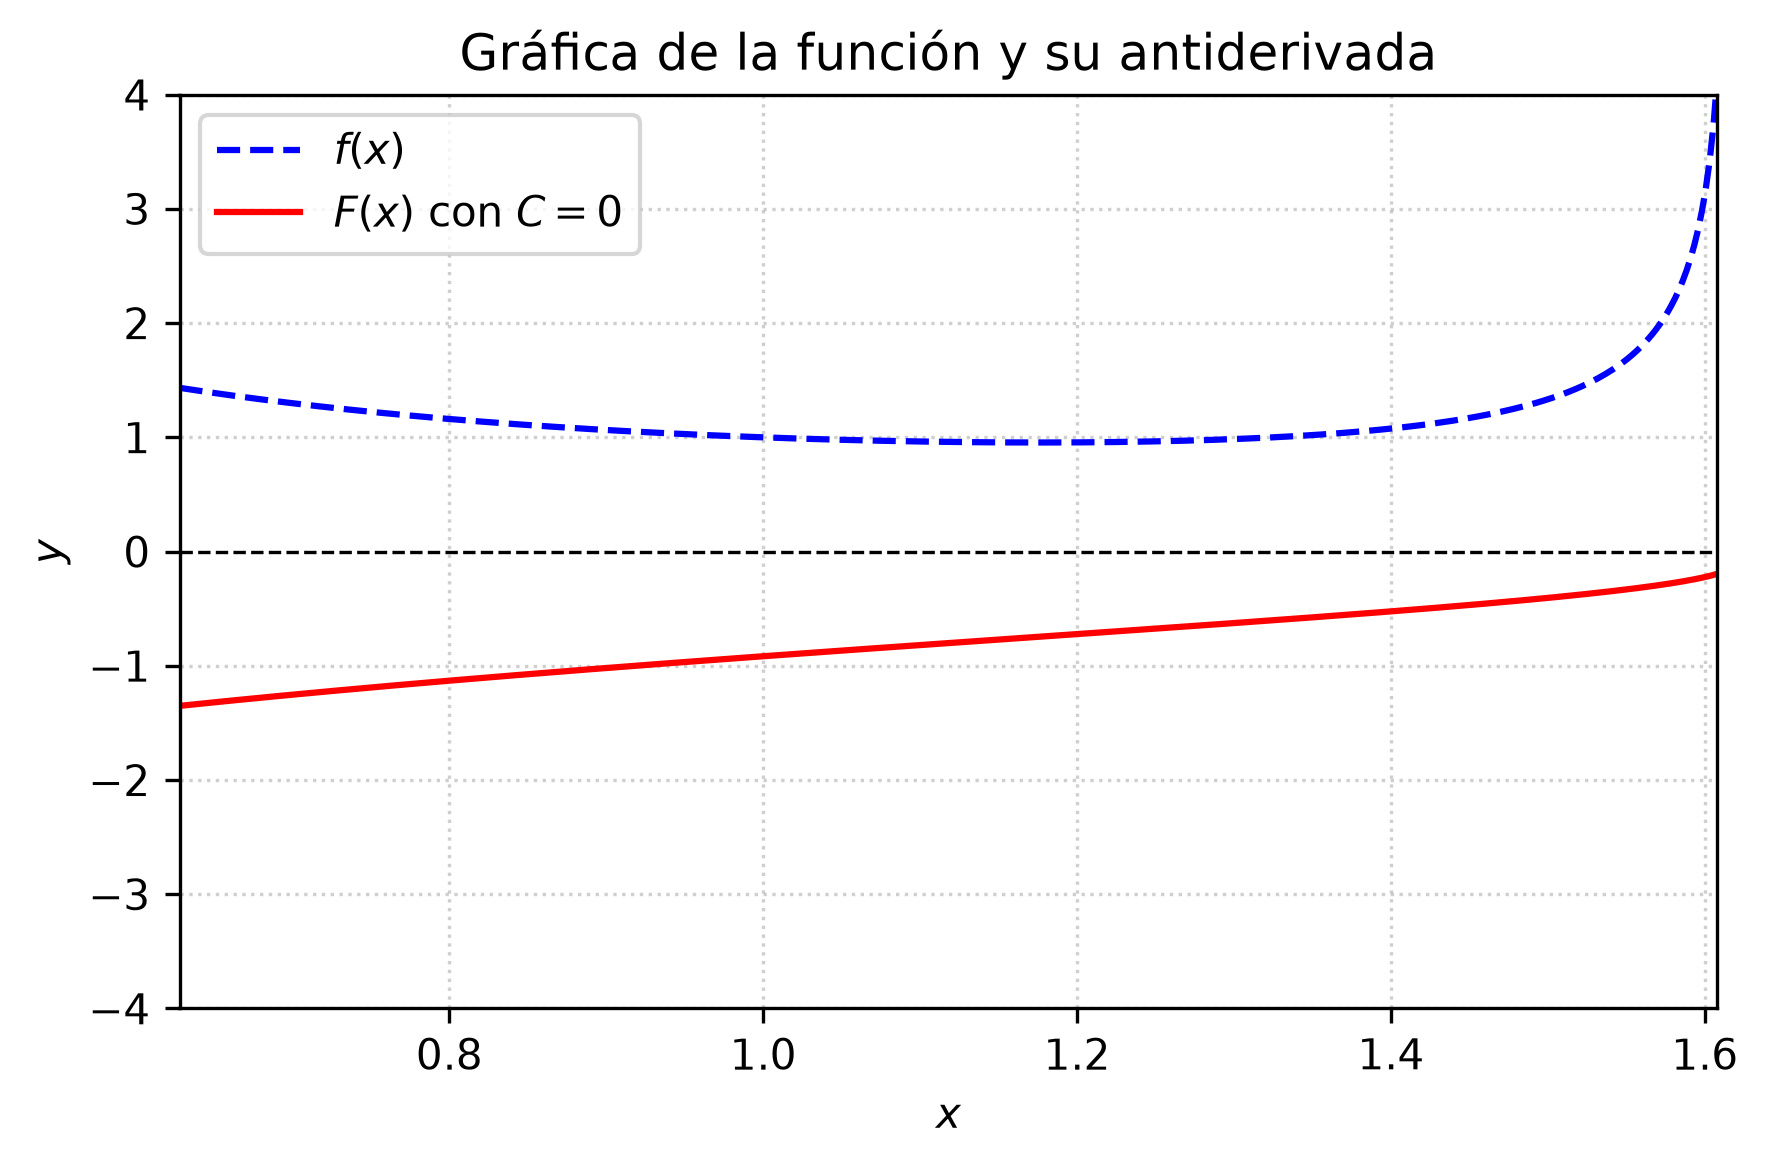
\includegraphics[width=\columnwidth]{semana_05/graficas/SEM05_P13_grafica.png}
	\caption{Representación gráfica de $f(x)$ y su antiderivada $F(x)$ evaluada para la constante de integración $C = 0$ (Problema 13).}
	\label{fig:problema13}
\end{figure}
